\documentclass[11pt, A4paper,norsk]{article}
\usepackage[utf8]{inputenc}
\usepackage[T1]{fontenc}
\usepackage{babel}
\usepackage{amsmath}
\usepackage{amsfonts}
\usepackage{amsthm}
\usepackage{amssymb}
\usepackage[colorlinks]{hyperref}
\usepackage{listings}
\usepackage{color}
\usepackage{hyperref}
\usepackage{graphicx}
\usepackage{cite}
\usepackage{textcomp}
\usepackage{float}

\definecolor{dkgreen}{rgb}{0,0.6,0}
\definecolor{gray}{rgb}{0.5,0.5,0.5}
\definecolor{daynineyellow}{rgb}{1.0,0.655,0.102}
\definecolor{url}{rgb}{0.1,0.1,0.4}

\lstset{frame=tb,
	language=Python,
	aboveskip=3mm,
	belowskip=3mm,
	showstringspaces=false,
	columns=flexible,
	basicstyle={\small\ttfamily},
	numbers=none,
	numberstyle=\tiny\color{gray},
	keywordstyle=\color{blue},
	commentstyle=\color{daynineyellow},
	stringstyle=\color{dkgreen},
	breaklines=true,
	breakatwhitespace=true,
	tabsize=3
}

\lstset{inputpath="C:/Users/Torstein/Documents/UiO/Fys3140/Python programmer"}
\graphicspath{{C:/Users/Torstein/Documents/UiO/Fys3140/"Python programmer"/}}
\hypersetup{colorlinks, urlcolor=url}

\author{Torstein Solheim Ølberg}
\title{Svar på Oblig nr. 13 i Fys3140}



%\lstinputlisting{Filnavn! type kodefil}
%\includegraphics[width=12.6cm,height=8cm]{Filnavn! type png}



\begin{document}
\maketitle
	\begin{center}
\Large \textbf{Oppgaver}
	\end{center}









		\paragraph{13.}
			\subparagraph{3.3)}
				\begin{flushleft}
Den initielle tilstandsfordelingen til temperaturen må tilfredstille Laplaces likning
$$\nabla^2 u_0 = \frac{d^2 u_0}{dx^2} = 0$$
$$u_0 = Ax + B$$
$$u_0(0) = 0 \Rightarrow B = 0$$
$$u_0(l) = 100 \Rightarrow A \cdot l = 100 \Rightarrow A = \frac{100}{l}$$
Etter dette tilfredstiller temperaturfordelingen varmelikningen. Da kan den tidsavhengige og posisjonsavhengige delen splittes til to funksjoner, der den tidsavhengige delen er gitt av uttrykket $T(t) = e^{- k^2 \alpha^2 t}$ og den posisjonsavhengige delen er gitt av likningen $\nabla^2 X + k^2 X = 0$ som i et endimensjonalt system har løsningen $X(x) = \sin(kx) \vee \cos(kx)$. Da blir den fulle likninga $u(x, t) = e^{- k^2 \alpha^2 t} \sin(kx) \vee  e^{- k^2 \alpha^2 t} \cos(k x)$. For å avgjøre hvilken av disse tilstandene vi skal bruke ser vi på grensebetingelsene. Begynner med $u(0, t) = 100$. Hvis vi bruker $\cos$ versjonen vil tidsdelen av likningen alltid være konstant, som virker veldig ulogisk, så derfor går vi for sinus hvor vi seinere kan legge på $100$ som en konstant for likningen, siden likningen vår nå blir null. Ser så på $u(l, t) = 0$. Da må enten $e^{- k^2 \alpha^2 t}$ eller $\sin(kl)$ være lik $0$
$$u(l, t) = e^{- k^2 \alpha^2 t} \sin(kl) = 0 \Rightarrow kl = n \pi$$
Siden tidsfuksjonen ikke burde være null velger vi at $kl = n \pi$. Da får vi at $k = \frac{n \pi}{l}$, som fører til
$$u(x, t) = e^{- \left( \frac{n \pi \alpha}{l} \right)^2 t} \sin\left( \frac{n \pi x}{l} \right)$$
Løsningen for dette problemet kan da skrives som serien under, med en ekstra lineær funksjon $u_f$ som representerer sluttstadiet. Denne funksjonen er da $100$ i $x = 0$ og $0$ i $x = l$
$$u(x, t) = \sum_{n = 1}^{\infty} b_n e^{- \left( \frac{n \pi \alpha}{l} \right)^2 t} \sin\left( \frac{n \pi x}{l} \right) + \left( 100 - \frac{100}{l}x \right)$$
Ved tiden $t = 0$ skal $u(x, 0)$ være lik $u_0$, så da får vi
$$\frac{100}{l}x - \left( 100 - \frac{100}{l}x \right) = \sum_{n = 1}^{\infty} b_n \sin\left( \frac{n \pi x}{l} \right)$$
$$\frac{200}{l}x - 100 = \sum_{n = 1}^{\infty} b_n \sin\left( \frac{n \pi x}{l} \right)$$
Vi kan da finne et uttrykk for $b_n$ ved å finne fourier koeffisienten en sinusserie av funksjonen $f(x) = \frac{200}{l}x - 100$. Denne koeffisienten er gitt ved
$$b_n = \frac{2}{l} \int_{0}^{l} f(x) \sin\left( \frac{n \pi x}{l} \right) dx$$
Putter så inn funksjonen vår, og finner et uttrykk for $b_n$
				\end{flushleft}
				\begin{gather*}
b_n = \frac{2}{l} \int_{0}^{l} \left( \frac{200}{l}x - 100 \right) \sin\left( \frac{n \pi x}{l} \right) dx \\
b_n = \frac{2}{l} \int_{0}^{l} \frac{200}{l}x \sin\left( \frac{n \pi x}{l} \right) dx - \frac{2}{l} \int_{0}^{l} 100 \sin\left( \frac{n \pi x}{l} \right) dx \\
b_n = \frac{2}{l} \frac{200}{l} \int_{0}^{l} x \sin\left( \frac{n \pi x}{l} \right) dx - \frac{2}{l} 100 \int_{0}^{l} \sin\left( \frac{n \pi x}{l} \right) dx \\
\text{Bruker sammenhengen $(121)$ fra Rotmann side $144$} \\
b_n = \frac{2}{l} \frac{200}{l}\left[ \frac{l^2}{n^2 \pi^2} \sin\left( \frac{n \pi x}{l} \right) - \frac{x l}{n \pi} \cos\left( \frac{n \pi x}{l} \right) \right]_{0}^{l} + \frac{2}{l} 100 \left[ \frac{l}{n \pi} \cos\left( \frac{n \pi x}{l} \right) \right]_{0}^{l} \\
b_n = \frac{400}{l^2} \left[ - \frac{l^2}{n \pi} \cos\left( n \pi \right) \right] + \frac{200}{l} \left[ \frac{l}{n \pi} \cos( n \pi ) - \frac{l}{n \pi} \cos(0) \right] \\
b_n = \frac{400}{n \pi} \left[ - \cos\left( n \pi \right) \right] + \frac{200}{n \pi} \left[ \cos( n \pi ) - 1 \right] \\
b_n = - \frac{200}{n \pi} \left[ \cos\left( n \pi \right) + 1 \right] \\
				\end{gather*}
				\begin{flushleft}
Setter dette inn i uttrykket for $u$ og får
$$u(x, t) = 100 - \frac{100}{l}x - \frac{200}{\pi} \sum_{n = 1}^{\infty} \frac{1}{n} \left( \cos\left( n \pi \right) + 1 \right) e^{- \left( \frac{n \pi \alpha}{l} \right)^2 t} \sin\left( \frac{n \pi x}{l} \right)$$
For alle $n$ som er oddetall blir parentesen med kosinus inni lik $0$ og for alle partall blir alle lik $2$. Derfor får vi
$$u(x, t) = 100 - \frac{100}{l}x - \frac{400}{\pi} \sum_{n = \text{partall}} \frac{1}{n} e^{- \left( \frac{n \pi \alpha}{l} \right)^2 t} \sin\left( \frac{n \pi x}{l} \right)$$
				\end{flushleft}








			\subparagraph{6.3)}
				\begin{flushleft}
Hvis vi ser på utslaget til en rektangulær membran som er festet langs alle sidene sine, vil dette uttrykket være $z(x, y, t)$. Vi kan separere dette uttryket i to fuksjoner, $z(x, y, t) = F(x, y)T(t)$. Dette skal tilfredstille bølgelikningen:
$$\nabla^2 F T = \frac{1}{v^2} \frac{\partial F T}{\partial t}$$
Dette kan skrives som en Helmholtz likning og en tidslikning
$$\nabla^2 F + K^2 F = 0 \wedge \ddot{T} + K^2 v^2 T = 0$$
Hvis vi da regner ut Helmholtz likningen blir dette
$$\frac{\partial^2 F}{\partial x^2} + \frac{\partial^2 F}{\partial y^2} + K^2 F = 0$$
Vi kan så prøve med å separere $x$ og $y$ i to forskjellige likninger.
$$F(x, y) = X(x) Y(y)$$
og vi får da likningen
$$Y \frac{\partial^2 X}{\partial x^2} + X \frac{\partial^2 Y}{\partial y^2} + K^2 X Y = 0 \Rightarrow \frac{1}{X} \frac{\partial^2 X}{\partial x^2} + \frac{1}{Y} \frac{\partial^2 Y}{\partial y^2} + K^2 = 0$$
Hvis vi splitter opp disse likningene får vi
$$\frac{\partial^2 X}{\partial x^2} + C^2 X = 0 \wedge \frac{\partial^2 Y}{\partial y^2} + (K^2 + C^2) Y = 0$$
Dette fører til at de to likningene får løsningene
$$X = \{ \sin(C x), \cos(C x) \} \wedge Y = \{ \sin(J x), \cos(J x) \}$$
der $J = \sqrt{K^2 - C^2}$. $T$ får løsningen $T = \{ \sin(K v t), \cos(K v t) \}$, altså blir den fulstendige løsningen
				\end{flushleft}
				\begin{gather*}
z(x, y, t) = X Y T = \left\{
\begin{tabular}{ c }
$\sin(C x)$ \\
$\cos(C x)$
\end{tabular}
\right\} \left\{
\begin{tabular}{ c }
$\sin(J y)$ \\
$\cos(J y)$
\end{tabular}
\right\} \left\{
\begin{tabular}{ c }
$\sin(Kv t)$ \\
$\cos(Kv t)$
\end{tabular}
\right\}
				\end{gather*}
				\begin{flushleft}
ved $x = 0$ skal utslaget bli $0$. Altså må $X$ være lik $\sin(C x)$. Samme gjelder når $y = 0$ så $Y = \sin(J y)$. For både $X$ og $Y$ blir konstantene lik $\frac{n \pi}{a} \wedge \frac{m \pi}{b}$.
$$J = \frac{m \pi}{b} = \sqrt{K^2 - \left( \frac{n \pi}{a} \right)^2}$$
$$K = \sqrt{\left( \frac{m \pi}{b} \right)^2 + \left( \frac{n \pi}{a} \right)^2}$$
				\end{flushleft}
				\begin{gather*}
z(x, y, t) = X Y T = \sin\left( \frac{n \pi x}{a} \right) \sin\left( \frac{m \pi y}{b} \right) \left\{
\begin{tabular}{ c }
	$\sin(Kv t)$ \\
	$\cos(Kv t)$
\end{tabular}
\right\}
				\end{gather*}
				\begin{flushleft}
Da blir $\nu = \frac{K v}{2 \pi} = \frac{v}{2 \pi} \sqrt{\left( \frac{m \pi}{b} \right)^2 + \left( \frac{n \pi}{a} \right)^2} = \frac{v}{2} \sqrt{\left( \frac{m}{b} \right)^2 + \left( \frac{n}{a} \right)^2}$
				\end{flushleft}
				\begin{figure}[H]
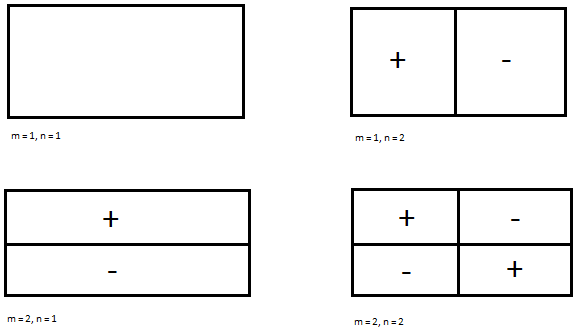
\includegraphics[width=12.6cm,height=9cm]{Skisse_13_1.png}
\caption{Skisse av normal modus vibrasjonene til en rektangulær membran.}
				\end{figure}
				\begin{flushleft}
Hvis vi nå ser på rektangelet som at det er kvadratisk blir likningen for frekvensene
$$\nu = \frac{v}{2} \sqrt{\left( \frac{m}{a} \right)^2 + \left( \frac{n}{a} \right)^2} = \frac{v}{2a} \sqrt{m^2 + n^2}$$
Da er det enkelt å se at så lenge $m_1^2 + n_1^2 = m_2^2 + n_2^2$ så er frekvensen $\nu$ vi får ut, den samme. Eksempler på dette kan være $m = 1, n = 7 \wedge m = 7, n = 1 \wedge m = 5, n = 5$. Alle disse tre fører til en frekvens $\nu = \frac{\sqrt{50} v}{2 a}$
				\end{flushleft}
				\begin{figure}[H]
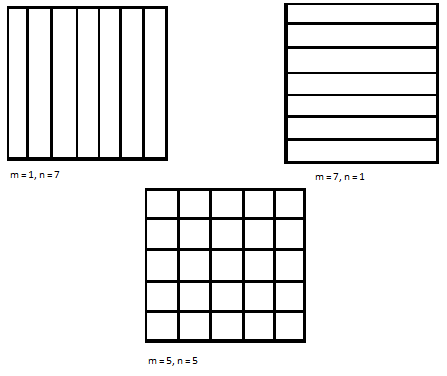
\includegraphics[width=12.6cm,height=10cm]{Skisse_13_2.png}
\caption{Skisse av normal modus vibrasjonene til en kvadratisk membran, der alle disse tre gir opphva til samme frekvens.}
				\end{figure}







			\subparagraph{c)}
				\begin{flushleft}
a
				\end{flushleft}
				\begin{gather}
a
				\end{gather}
			









			\subparagraph{d)}
				\begin{flushleft}
a
				\end{flushleft}










			\subparagraph{e)}
				\begin{flushleft}
a
				\end{flushleft}









		\paragraph{2.}
			\subparagraph{a)}
				\begin{flushleft}
a
				\end{flushleft}









			\subparagraph{b)}
				\begin{flushleft}
a
				\end{flushleft}












			\subparagraph{c)}
				\begin{flushleft}
a
				\end{flushleft}












			\subparagraph{d)}
				\begin{flushleft}
a
				\end{flushleft}









			\subparagraph{e)}
				\begin{flushleft}
a
				\end{flushleft}










			\subparagraph{f)}
				\begin{flushleft}
a
				\end{flushleft}








			\subparagraph{g)}
				\begin{flushleft}
a
				\end{flushleft}









			\subparagraph{h)}
				\begin{flushleft}
a
				\end{flushleft}
\end{document}